\documentclass{article}
\usepackage[utf8]{inputenc}
\usepackage{tikz}
\usepackage{graphicx}
\usepackage{amsmath}
\usetikzlibrary{shapes.geometric, arrows}

\tikzstyle{startstop1} =
[
	rectangle
	, text width=2cm
	, minimum height=0.8cm
	, text badly centered
	, draw=black
	, fill=white
]
\tikzstyle{process1}= 
[
	rectangle
	, text width=3.4cm
	, minimum height=0.8cm
	, draw=black
	, fill=white
]
\tikzstyle{process2}= 
[	
	rectangle
	, text width=2.5cm
	, minimum height=0.8cm
	, draw=black
	, fill=white
]
\tikzstyle{process3}=
[
	rectangle
	,rounded corners
	,minimum width=4cm
	,text height=0.35cm
	,draw=black
	,fill=white
	,text centered
]
\tikzstyle{hinhthoi1}=
[
	diamond
	,text width=3cm
	,text height=0
	,text centered
	,draw=black
	,fill=white
] 
\tikzstyle{khongvien}=
[
	rectangle
	,text centered
	,minimum width=0cm
	,minimum height=0cm
	,draw=white
	,fill=white
]

\tikzstyle{arrow} = [thick,->,>=stealth]
\tikzstyle{line} = [thick,-]

\begin{document}

%FIGURE 7
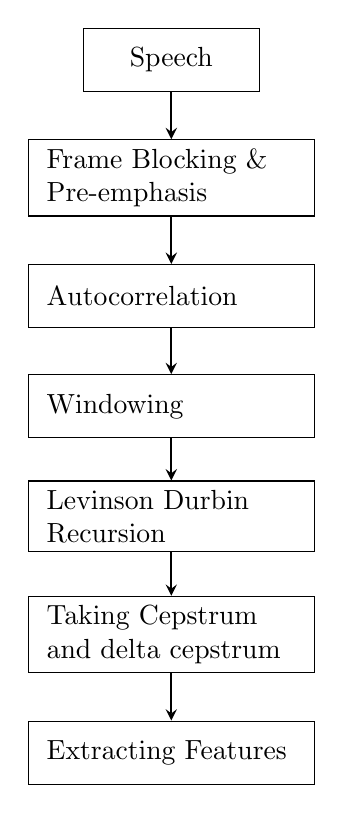
\begin{tikzpicture}[node distance=1.5cm]

\node(start)[startstop1]{Speech};
\node(pro1)[process1, below of=start]{\ Frame Blocking \& \\ \ Pre-emphasis};
\node(pro2)[process1, below of=pro1]{\ Autocorrelation};
\node(pro3)[process1, below of=pro2, yshift=0.1cm]{\ Windowing};
\node(pro4)[process1, below of=pro3, yshift=0.1cm]{\ Levinson Durbin \\ \ Recursion};
\node(pro5)[process1, below of=pro4]{\ Taking Cepstrum \\ \ and delta cepstrum};
\node(pro6)[process1, below of=pro5]{\ Extracting Features};

\draw[arrow](start)--(pro1);
\draw[arrow](pro1)--(pro2);
\draw[arrow](pro2)--(pro3);
\draw[arrow](pro3)--(pro4);
\draw[arrow](pro4)--(pro5);
\draw[arrow](pro5)--(pro6);

\end{tikzpicture}
                  
%FIGURE 8
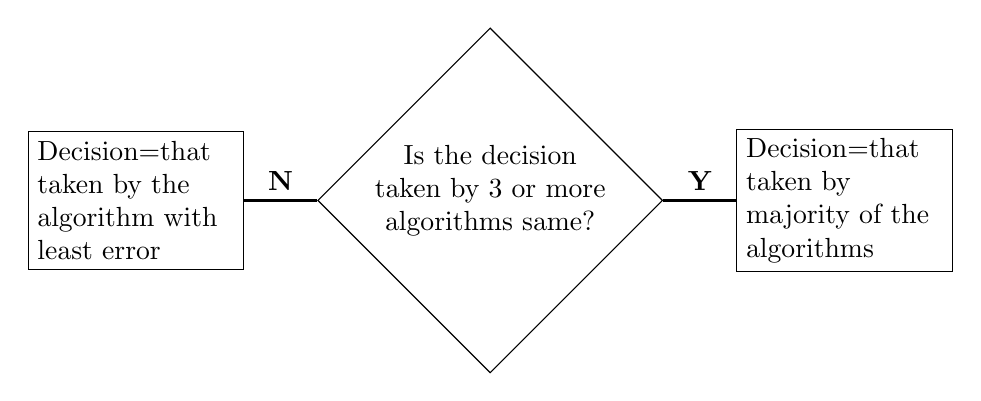
\begin{tikzpicture}[node distance=4.5cm]

\node(hinhthoi)[hinhthoi1]{Is the decision taken by 3 or more algorithms same?};
\node(pro1)[process2, left of=hinhthoi]{Decision=that taken by the algorithm with least error};
\node(pro2)[process2, right of=hinhthoi]{Decision=that taken by \\ majority of the algorithms};

\draw[line](hinhthoi)--node[anchor=south]{\bfseries N}(pro1);
\draw[line](hinhthoi)--node[anchor=south]{\bfseries Y}(pro2);

\end{tikzpicture}

%FIGURE 4
\begin{tikzpicture}[node distance=0.85cm,auto]

\node(pro1)[process3]{Signal frame=s};
\node(arrow1)[khongvien, below of=pro1,node distance=0.8cm]{\includegraphics[scale=0.75]{arrow1.png}};
\node(pro2)[process3,below of=arrow1]{S = DFT(s)};
\node(arrow2)[khongvien, below of=pro2]{\includegraphics[scale=0.75]{arrow1.png}};
\node(pro3)[process3, below of=arrow2]{PSD = $|\text{S}|^2$};
\node(arrow3)[khongvien, below of=pro3]{\includegraphics[scale=0.75]{arrow1.png}};
\node(pro4)[process3, below of=arrow3]{ApplyMel filterbank};
\node(arrow4)[khongvien, below of=pro4]{\includegraphics[scale=0.75]{arrow1.png}};
\node(pro5)[process3, below of=arrow4]{\ \ \ obtain total energy in each filterbank\ \ \ };
\node(arrow5)[khongvien, below of=pro5]{\includegraphics[scale=0.75]{arrow1.png}};
\node(pro6)[process3, below of=arrow5]{\ \ \ Take natural logarithm of energies\ \ \ };
\node(arrow6)[khongvien, below of=pro6]{\includegraphics[scale=0.75]{arrow1.png}};
\node(pro7)[process3, below of=arrow6]{\ \ \ Take DCT of log energies\ \ \ };
\node(arrow7)[khongvien, below of=pro7]{\includegraphics[scale=0.75]{arrow1.png}};
\node(pro8)[process3, below of=arrow7]{\ \ \ Keep first 13 coefficients\ \ \ };

\end{tikzpicture}

%FIGURE 6

\end{document}
%\makebox[\linewidth][c]{ } : cho cái trong ngoặc vào giữa
% rounded corners : làm mềm góc 
